\documentclass{standalone}
\usepackage[T1]{fontenc}
\usepackage[utf8]{inputenc}
\usepackage[english]{babel}
\usepackage{tikz}
\usetikzlibrary{calc,through,backgrounds,positioning,fit,mindmap}
\usetikzlibrary{shapes,arrows,shadows}
 
\begin{document}
 
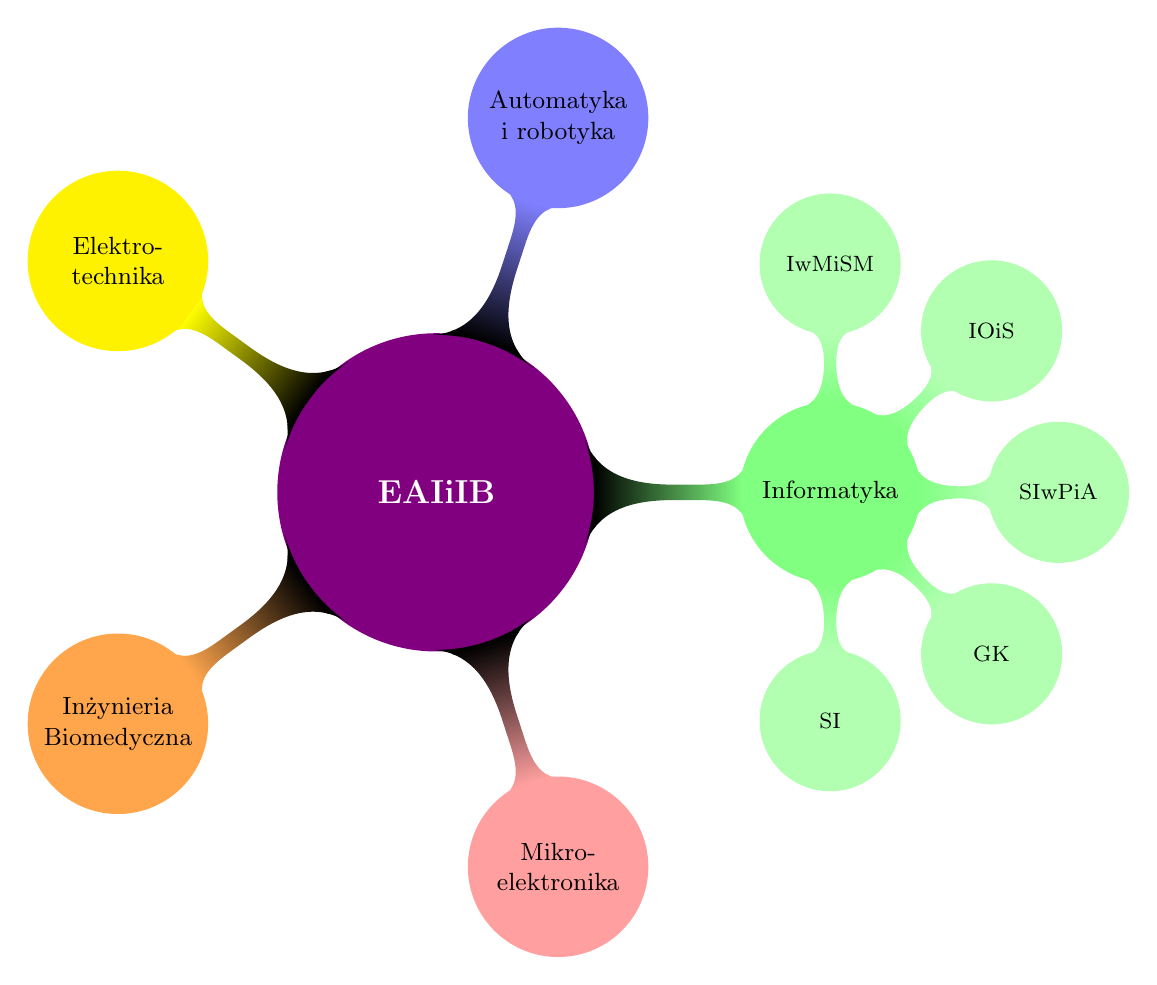
\begin{tikzpicture}[mindmap]
\node [concept,concept color=red!50!blue, text=white] {\bf EAIiIB}
  child[grow=0, concept color=green!50] {node[concept] {Informatyka}
    child[grow=90, concept color=green!30] {node[concept] {IwMiSM}}
    child[grow=45, concept color=green!30] {node[concept] {IOiS}}
    child[grow=0, concept color=green!30] {node[concept] {SIwPiA}}
    child[grow=-45, concept color=green!30] {node[concept] {GK}}
    child[grow=-90, concept color=green!30] {node[concept] {SI}}
  }
  child[grow=72, concept color=blue!50] {node[concept] {Automatyka i robotyka}}
  child[grow=144, concept color=yellow!100] {node[concept] {Elektro- technika}}
  child[grow=216, concept color=orange!70] {node[concept] {Inżynieria Biomedyczna}}
  child[grow=288, concept color=pink!150] {node[concept] {Mikro- elektronika}}
  ;
\end{tikzpicture}
 
\end{document}